\chapter{Monitoring System Architecture}
\label{chap:Monitoring System Architecture}

In this chapter we describe the high-level structure of our proposed monitoring system, why we chose this architecture, it's benefits, followed by some lessons we learned during development.

\section{High-Level Architecture}
\label{sec:Architecture}

The monitoring system will use the Xposed framework to inject code into all processes running on Android. The code will report on interesting process activities.  Android's effective process separation restricts each process to only being able to report on its own activity, but in order to recognise collusion between many, it is necessary to gather all reports into a single trace.  Naturally, this promotes an architecture where many processes report their activity to a single process responsible for maintaining the trace and monitoring the activity.  Implementation, therefore, falls into two halves; an interceptor module and a monitor.  Further restraints imposed by Android on inter-process communication encourage the intent system as the means of communication between the two halves.

Figure \ref{fig:highLevelArchitectureDiagram} illustrates the architecture: The bottom of the diagram shows the installed applications that are not yet executing.  The top depicts applications launched by the user.  The executing applications have the interceptor module injected and report their activity to a single monitor process via a designated intent channel.

\begin{figure}[h]
  \centering
  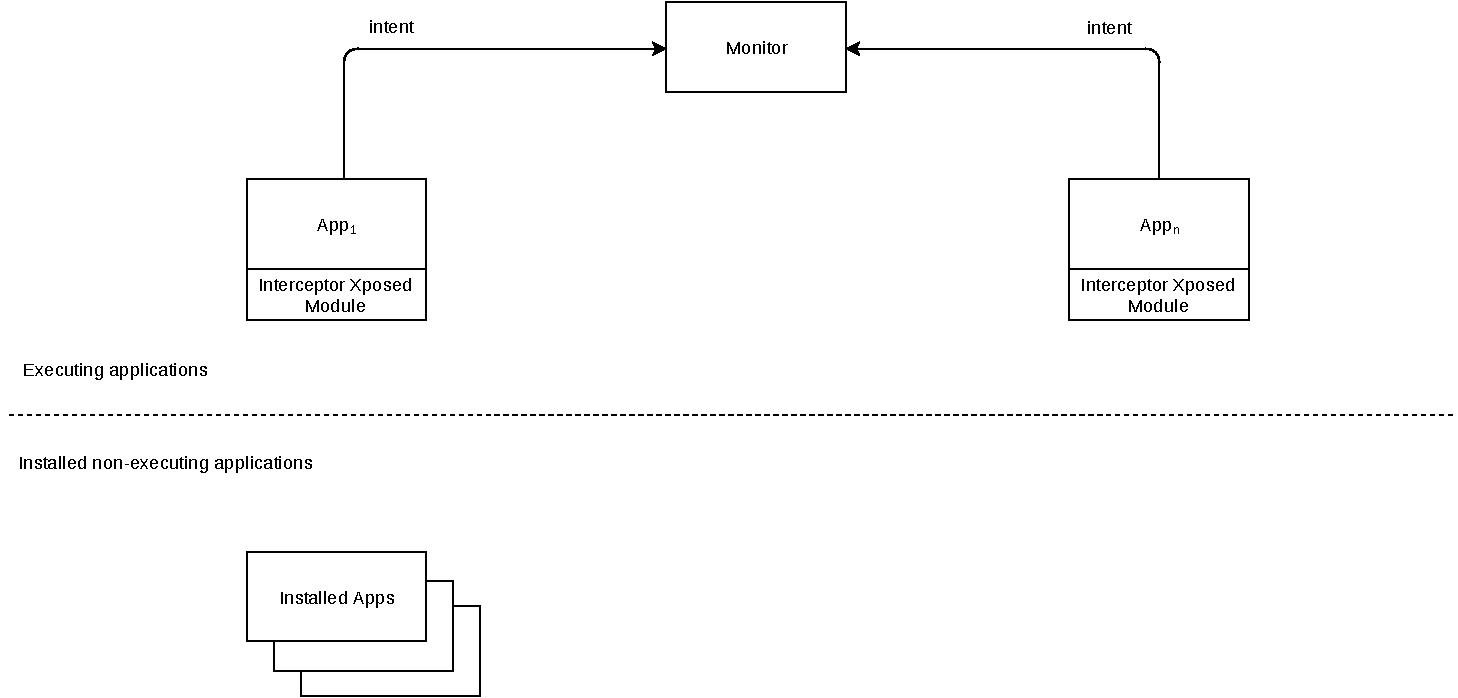
\includegraphics[width=\textwidth]{graphics/HighLevelArchitecture.pdf}
  \caption{High Level Architecture Diagram}
  \label{fig:highLevelArchitectureDiagram}
\end{figure}

\FloatBarrier

\section{Interceptor}
\label{sec:Interceptor}

The first part of the monitoring system is an Xposed module called the interceptor.  Figure \ref{fig:interceptorClassDiagram} below shows the structure.  The interceptor contains callback classes derived from XC\_MethodHook that Xposed hooks to interesting operating system methods.  Whenever a hooked method is called, the callback is invoked first, then the O/S method will be allowed to continue as usual.

The Xposed framework injects the callbacks into every process, therefore intercepted O/S calls will be from every process.  In order to recognise collusion between different applications, we must gather the details of the calls into a single trace.  Callbacks do this by capturing details of the method calls and notifying a single monitor process via an Android intent.

It is relevant now to mention a quirk that leads to a hazard we must avoid.  Xposed will inform the interceptor of its own attempt to send an intent to the monitor.  In addition, the monitor process will have the interceptor module injected into it.\footnote{This technicality is omitted from figure \ref{fig:highLevelArchitectureDiagram}.}  If the monitor system reports on its own activity, we hit the halting problem.  Of course, the interceptor knows the intent channel designated for communication to the monitor, so it ignores communication over that intent. 

Figure \ref{fig:interceptorClassDiagram} below shows five classes derived from XC\_MethodHook, one for each of the methods of interest identified in section \ref{sec:OSMethodsOfInterest}.  The MethodHooks class implements IXposedHookLoadPackage.handleLoadPackage() that is invoked whenever any process requires a package to be loaded.  If the package contains one of the operating system methods we are interested in, then the corresponding XC\_MethodHook class will be created and registered with Xposed.  Then, whenever the host process calls the interesting operating system method, beforeHookedMethod() will be called on the XC\_MethodHook class, and the interceptor will notify the monitor.

\begin{figure}[h]
  \centering
  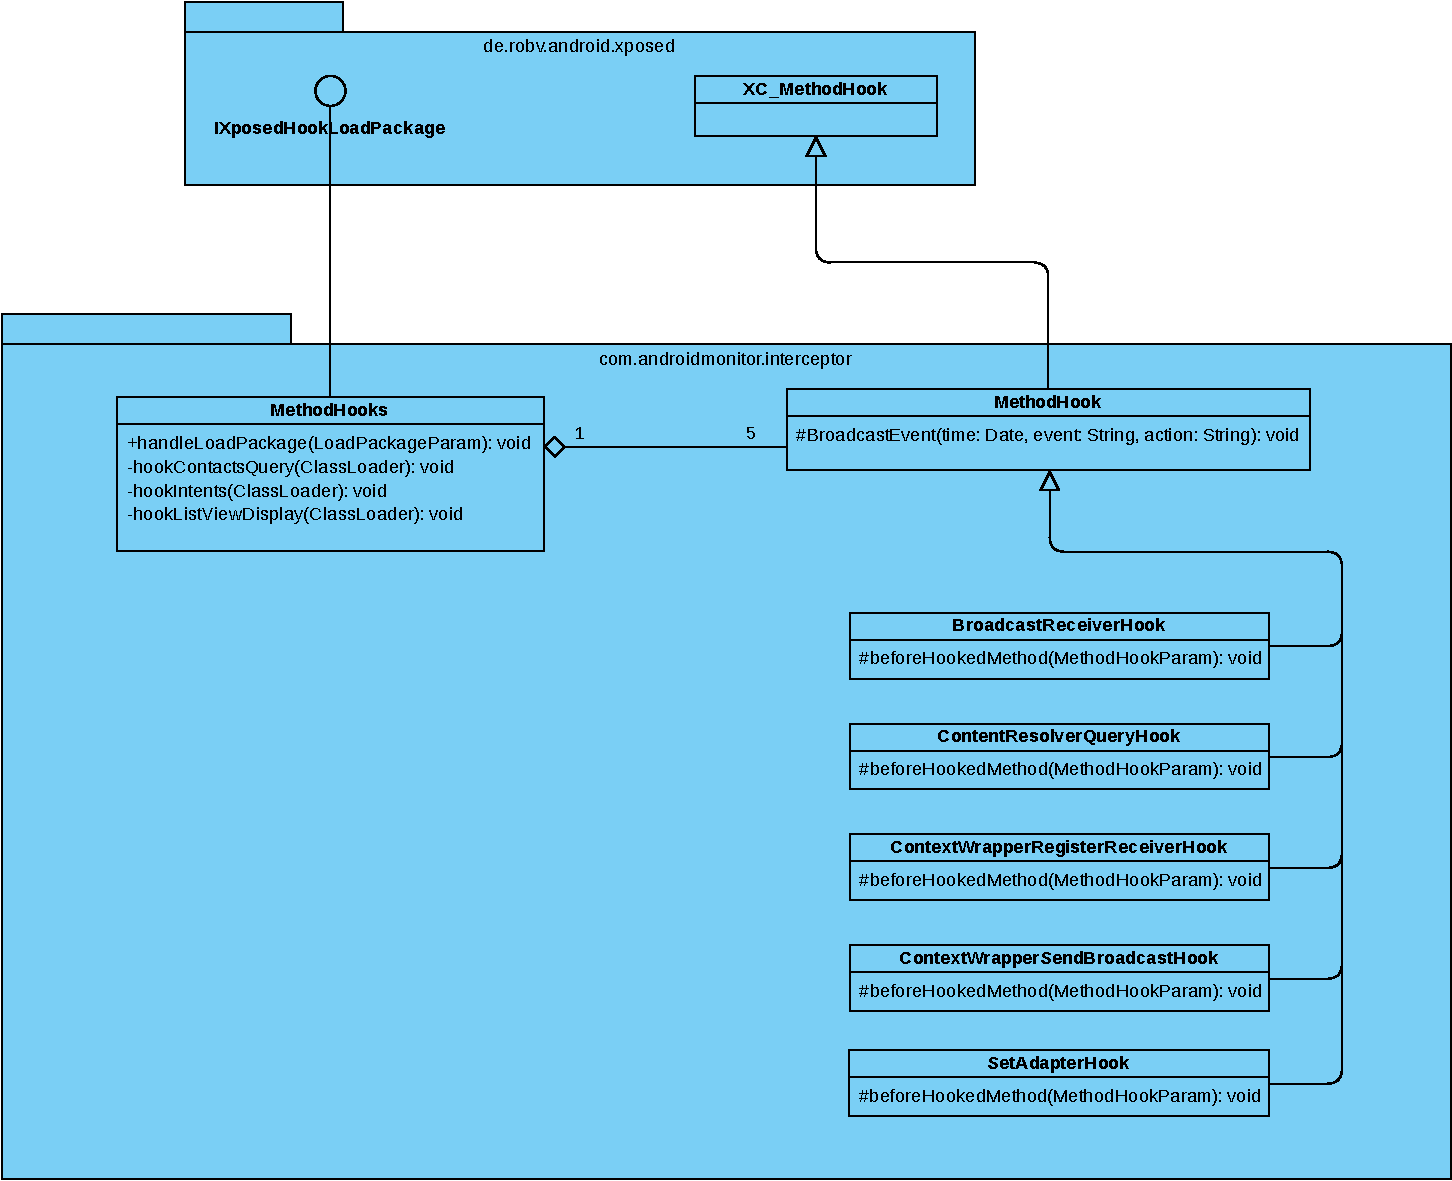
\includegraphics[width=\textwidth]{graphics/InterceptorClassDiagram.pdf}
  \caption{Interceptor Class Diagram}
  \label{fig:interceptorClassDiagram}
\end{figure}

\section{Monitor}
\label{sec:Monitor}

The second half of the system is the monitor.  The monitor receives intents from the interceptor, the details of the O/S call get extracted, put into an event, then passed to an instance of the \RH\ algorithm.  The event gets evaluated to determine if the formula is satisfied and if so, the monitor alerts the user that some malicious activity may have taken place.  The monitor could evaluate different formulae simultaneously by constructing multiple algorithm instances, one for each formula.  For now, we only evaluate the collusion formula.

\section{Benefits}
\label{sec:Benefits}

There is an added advantage to separating activity reporting from monitoring.  The intensive work for the developer is in evaluating the trace for the satisfaction of LTL formulae.  Whereas the reporting of activities is relatively straightforward.  Furthermore, once interesting O/S methods have been identified, and there is code implemented to intercept them, that code requires little maintenance.  This is a great benefit because the interceptor becomes the only part of the system dependent on the Xposed framework.

Development with this framework has proved awkward because of its nature.  The Xposed module code gets injected into the Android zygote process on boot-up of Android.  For a module to take effect, it is necessary to reboot the device after the module gets installed.  Alterations to the module require the previous version to be uninstalled, the new version installed, and the device rebooted.  Not only does this slow the development cycle, but there are two important consequences:  Any faults in an Xposed module can result in Android failing to boot.  It is then impossible to remove the Xposed module because it can only be uninstalled using an administration tool launched within Android.  If Android does not boot, then the administration tool cannot be used to uninstall the faulty Xposed module.  The device is 'bricked'.

Experience has shown that developing on a virtual Android device and keeping a backup of it with all necessary development tools pre-installed is very prudent.  Faulty Xposed modules have also proved impossible to debug using standard debugging tools because the code begins executing on boot-up of Android rather than being launched once Android is running.  It is necessary to attach the debug tool to running processes, but this has been unsuccessful so far.  The upshot is that debugging tools that allow the developer to stop execution at a breakpoint within the code, trace through the code and inspect memory are unusable.  The risk of bricking the device during development makes all but the simplest code infeasible as an Xposed module.

Thankfully, if the Xposed module only intercepts interesting methods, then it is kept simple.  Once the module is complete, it does not require maintenance so development cycles are kept rapid.  It follows that the complex work falls into the monitor half of the system, where it is easier to debug and cannot render the device unusable.  We describe the structure of the monitor in later chapters \ref{chap:Runtime Verification with the Rosu-Havelund Algorithm} and \ref{chap:Reverse Rosu-Havelund Algorithm}.
